\chapter{ Desarrollo software }
\label{chap:desarrollo-software}


\section{Metodología de desarrollo}

Este proyecto ha sido obtenido empleando una metodología de desarrollo basada en
el modelo de desarrollo incremental para la parte software referente a todos los subsistemas web y una metodología de desarrollo en cascada para el desarrollo de la parte
software del robot de pruebas.\\

El modelo de desarrollo incremental proporciona una serie de características que lo hacen idóneo para este proyecto. Dicho modelo se basa en la filosofía de construir 
e ir incrementando las funcionalidades del sistema mediante el desarrollo de los diferentes módulos. Esto permite ir aumentando gradualmente las capacidades del software. \\

Dicha metodología de desarrollo resulta especialmente útil en las siguientes situaciones:\\

\begin{itemize}
 \item Facilita el desarrollo permitiendo a cada miembro del equipo desarrollar un módulo particular. En el caso del presente proyecto me ha permitido desarrollar un módulo tras otro de una manera secuencial.
 \item Es similar al ciclo de vida en cascada aplicándose un ciclo en cada nueva funcionalidad del programa.
 \item A final de cada ciclo se entrega el software al cliente. En el caso que compete a este proyecto se mantenía una reunión con el director del proyecto para su aprobación.
\end{itemize}

Por otro lado, el modelo de desarrollo en cascada resulta adecuado en situaciones en las que:\\

\begin{itemize}
 \item Se dispone de unos requisitos claros y precisos.
 \item El sistema a desarrollar es de pequeña envergadura.
 \item Las tecnologías utilizadas son conocidas por los desarrolladores.
\end{itemize}


Centrándonos nuevamente en el desarrollo del proyecto, los motivos que llevaron a cabo la elección de un modelo de desarrollo incremental viene dada por la necesidad de simplificar e ir
desarrollando de una forma gradual y modularizada debido a la extensión del proyecto. Más si cabe que el equipo de desarrollo solo consta de una persona.\\

Por otro lado, para el desarrollo del vehículo de pruebas y por su simplicidad, se ha optado por un desarrollo en cascada además de que en otras ocasiones ya había realizado trabajos similares.\\

Por tanto el proyecto queda distribuido en los siguientes subsistemas:\\

\begin{figure}[H]
  \begin{center}
    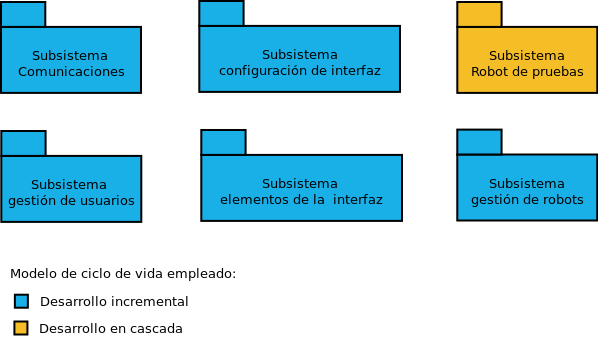
\includegraphics[scale=.6]{diagramas/subsistemas.png}
  \end{center}
  \caption{Subsistemas existentes en el proyecto junto con el modelo de ciclo de vida
utilizado para su desarrollo.}
  \label{website:pagina-principal}
\end{figure}


\section{Recolección de requisitos}

\subsection{Requisitos funcionales}

Para la elaboración de este proyecto se ha utilizado la metodología Métrica V3 así como el estándar ISO/IEC 12207. Métrica es una metodología de planificación, desarrollo y
mantenimiento de los sistemas de información desarrollada por el Ministerio de Administraciones Públicas del Gobierno de España. Tiene como objetivo proporcionar una guía para 
la sistematización de actividades del ciclo de vida de los proyectos software en el ámbito de las administraciones públicas.\\

Métrica V3 \cite{website:metrica} está basada en el modelo de procesos del ciclo de vida de desarrollo ISO/IEC 12207 (Information Technology - Software Life Cycle Processes) así como
en la norma ISO/IEC 15504 SPICE (Software Process Improvement And Assurance Standards Capability Determination).\\

En la página oficial de Métrica V3, sus desarrolladores indican que puede ser utilizada libremente con la única restricción de citar la fuente de su propiedad intelectual, 
la del Ministerio de Administraciones Públicas.\\

En esta etapa del modelado de requisitos se captura el propósito general del sistema:

\begin{itemize}
  \item Se analiza qué debe hacer el sistema.
  \item Se obtiene una versión contextualizada del sistema.
  \item Identifica y delimita el sistema.
  \item Se determinan las características, cualidades y restricciones que debe satisfacer el sistema.
\end{itemize}


Por tanto, Los requisitos funcionales que se han obtenido después del proceso de obtención de requisitos son:\\

\begin{itemize}
  \item Definir los pasos para dar de alta un dispositivo robótico en el sistema.
  \item Una vez configurado el dispositivo, configurar la interfaz de control con las acciones de control específicas.
  \item Realizar un sistema de monitorización y visualización para los usuarios y los dispositivos robóticos en tiempo real.
  \item Sistema de gestión de base de datos en donde se encuentren los datos de la aplicación recogidos.
  \item Disponer de un panel de administración donde visualizar la información de los usuarios conectados y dispositivos en uso en tiempo real. 
  \item Proporcionar un sistema de streaming de vídeo para la difusión de imágenes a los usuarios espectadores procedentes de los robots dispongan de cámara.
  \item Deberá ser una herramienta multiplataforma.  
\end{itemize}



\subsection{Requisitos no funcionales}

Los requisitos no funcionales son aquellos que describen cualidades o restricciones del sistema que no se relacionan de forma directa con el comportamiento funcional del mismo. A continuación se especifican los más importantes del sistema:
\begin{itemize}
\item No requiere un conocimiento específico del sistema una vez puesto en funcionamiento.
\item La aplicación tendrá manual de uso.
\item La base de datos estará implementada en un lenguaje objeto no relacional como MongoDB.
\item La aplicación estará realizada en el lenguaje de programación Python.
\item La interfaz debe reflejar claramente la distinción entre las distintas partes del sistema.
\item El sistema se desplegará sobre una versión GNU Linux Debian 8 Jessie.
\item El código fuente de la aplicación seguirá un estilo uniforme y normalizado para todos los módulos del mismo.
\end{itemize}


\section {Diagramas de casos de uso}

Un caso de uso es una descripción de los pasos o actividades que deberán realizarse para llevar a cabo algún proceso. Los objetivos de los casos de uso son los siguientes:

\begin{itemize}
\item Obtener los requisitos funcionales del sistema y expresarlos desde un punto de vista más cercano al usuario.
\item Proporcionar una guía de todo el proceso de desarrollo del sistema de información. Los casos de uso proporcionan, por tanto, un modo claro y preciso de comunicación entre lo que desea el cliente y el desarrollador proporcionando desde el punto de vista del cliente una visión de ``caja negra'' del sistema eliminando los detalles de su construcción o desarrollo. Para los desarrolladores es utilizado como punto de partida y el eje sobre el que se apoya todo el desarrollo del sistema en los procesos de análisis y diseño.
\end{itemize}

Los diagramas de caso de uso muestra una representación del comportamiento ofrecido por el sistema de información desde el punto de vista del usuario. El comportamiento
del sistema es representado como un conjunto de transacciones ejecutadas entre el sistema y los actores junto con la descripción sobre las de las relaciones de comunicación
existentes entre un actor y el sistema.\\

En la figura \ref{diagram:caso-uso} podemos observar los diagramas de casos de uso resultantes tras la recolección de requisitos:

\begin{figure}[H]
  \begin{center}
    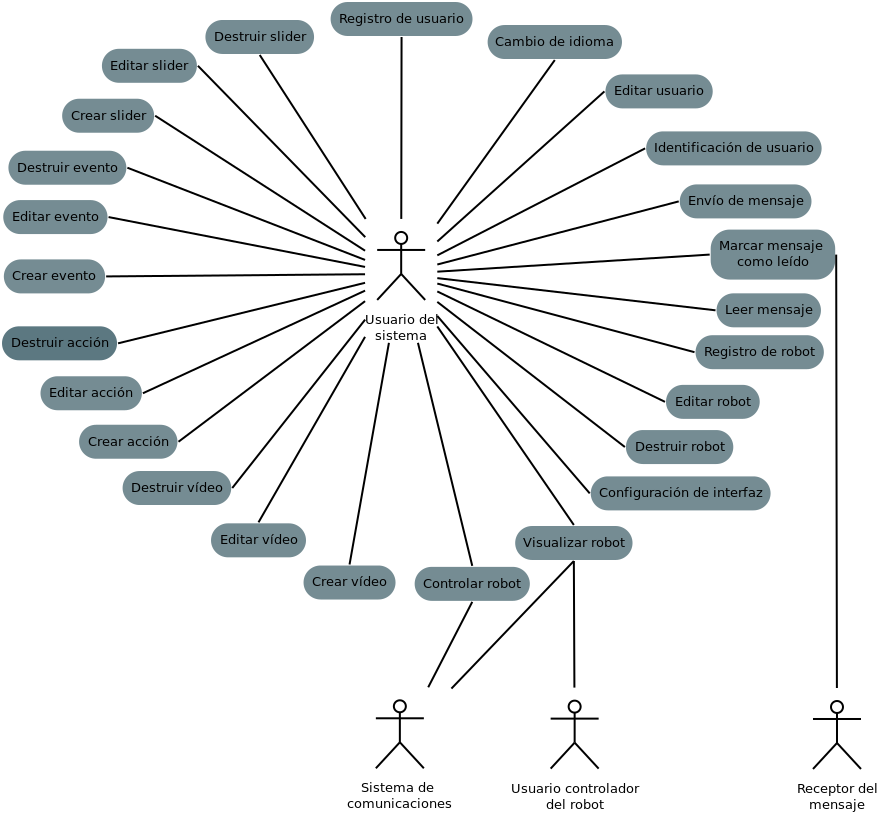
\includegraphics[scale=.5]{diagramas/casos-uso.png}
  \end{center}
  \caption{Diagrama de casos de uso para la interacción con la aplicación.}
  \label{diagram:caso-uso}
\end{figure}




\begin{figure}[H]
  \begin{center}
    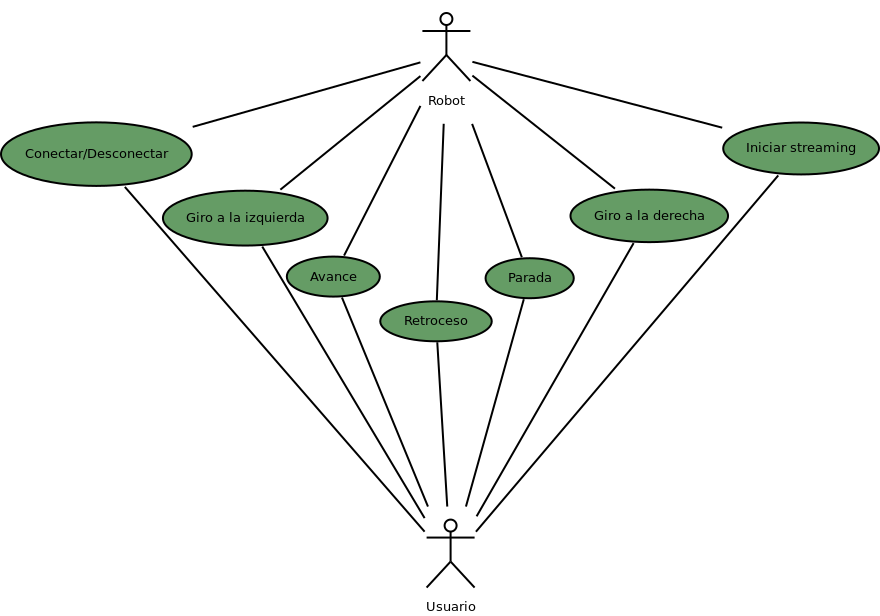
\includegraphics[scale=.5]{diagramas/casos-uso-robot.png}
  \end{center}
  \caption{Diagrama de casos de uso para la interacción con el robot de pruebas.}
  \label{diagram:caso-uso}
\end{figure}





\section{Especificación de los casos de uso}
\label{sec:especificaciones-caso-uso}


A continuación se proporciona la especificaciones de cada uno de los casos de uso de la figura \ref{diagram:caso-uso}:


\begin{table}[H]
  \begin{center}
    \begin{tabular}{|p{3.5cm}|p{10cm}|}
      \hline
      {\textbf{Caso de uso:}} & { Registro de usuario.} \\
      \hline
      {\textbf{Descripción:}} & { El sistema deberá actuar como describe en este caso de uso cuando el usuario solicita el registro en el sistema.} \\
     \hline
      {\textbf{Actor principal:}} & { Usuario del sistema.} \\
      \hline
      {\textbf{Actor secundario:}} & { - } \\
      \hline
      {\textbf{Precondiciones:}} & { - } \\
     \hline   
    {\textbf{Flujo principal:}} & { 
      \begin{enumerate}
	\item El actor usuario del sistema solicita el registro en el sistema.
	\item El sistema solicita los datos correo electrónico, nombre de usuario, avatar, contraseña, confirmación de contraseña e idioma.
	\item El usuario proporciona al sistema al menos los siguientes datos, correo electrónico, nombre de usuario, contraseña y confirmación de contraseña.
	\item El sistema realiza el registro de un nuevo usuario e informa de que el registro se ha realizado con éxito.
      \end{enumerate}
      } \\
     \hline
     {\textbf{Postcondición}} & {Se realiza el registro de un usuario en el sistema.}\\
     \hline
         {\textbf{Excepciones:}} & {
         \begin{enumerate}
          \item Si existe un usuario con el correo electrónico introducido:
          \begin{itemize}
           \item El sistema informa de que no se puede realizar el registro.
           \item Se cancela el caso de uso.
          \end{itemize}
	  \item Si la contraseña y la confirmación no coinciden:
	    \begin{itemize}
	      \item El sistema informa de que no se puede realizar el registro.
	      \item Se cancela el caso de uso.
	    \end{itemize}
         \end{enumerate}
         }\\
     \hline
    \end{tabular}
  \end{center}
\caption{Descripción del caso de uso: Registro de usuario.}
\end{table}




\begin{table}[H]
  \begin{center}
    \begin{tabular}{|p{3.5cm}|p{10cm}|}
      \hline
      {\textbf{Caso de uso:}} & { Identificación de usuario.} \\
      \hline
      {\textbf{Descripción:}} & { El sistema deberá actuar como describe en este caso de uso cuando el usuario solicita la Identificación en el sistema.} \\
     \hline
      {\textbf{Actor principal:}} & { Usuario del sistema.} \\
      \hline
      {\textbf{Actor secundario:}} & { - } \\
      \hline
      {\textbf{Precondiciones:}} & { El usuario debe estar registrado en el sistema } \\
     \hline   
    {\textbf{Flujo principal:}} & { 
      \begin{enumerate}
	\item El actor usuario del sistema solicita la Identificación en el sistema.
	\item El sistema solicita los datos correo electrónico y contraseña.
	\item El usuario proporciona al sistema el correo electrónico y contraseña.
	\item El sistema realiza el logueo del usuario y crea una sesión.
      \end{enumerate}
      } \\
     \hline
     {\textbf{Postcondición}} & {Se realiza la identificación del usuario en el sistema, se crea una sesión y se carga el idioma establecido por el usuario.}\\
     \hline
         {\textbf{Excepciones:}} & {
         \begin{enumerate}
          \item Si no existe un usuario con el correo electrónico introducido:
          \begin{itemize}
           \item El sistema informa de que no existe ningún usuario con ese correo electrónico.
           \item Se cancela el caso de uso.
          \end{itemize}
	  \item Si la contraseña es incorrecta:
	    \begin{itemize}
	      \item El sistema informa de que la contraseña es incorrecta.
	      \item Se cancela el caso de uso.
	    \end{itemize}
         \end{enumerate}
         }\\
     \hline
    \end{tabular}
  \end{center}
\caption{Descripción del caso de uso: Identificación de usuario.}
\end{table}


\begin{table}[H]
  \begin{center}
    \begin{tabular}{|p{3.5cm}|p{10cm}|}
      \hline
      {\textbf{Caso de uso:}} & { Cambio de idioma.} \\
      \hline
      {\textbf{Descripción:}} & { El sistema deberá actuar como describe en este caso de uso cuando el usuario solicita cambiar de idioma la página.} \\
     \hline
      {\textbf{Actor principal:}} & { Usuario del sistema.} \\
      \hline
      {\textbf{Actor secundario:}} & { - } \\
      \hline
      {\textbf{Precondiciones:}} & { - } \\
     \hline   
    {\textbf{Flujo principal:}} & { 
      \begin{enumerate}
	\item El actor usuario del sistema selecciona un idioma disponible.
	\item El sistema establece el idioma seleccionado.
      \end{enumerate}
      } \\
     \hline
     {\textbf{Postcondición}} & {Se realiza el cambio de idioma en la aplicación.}\\
     \hline
         {\textbf{Excepciones:}} & { - }\\
     \hline
    \end{tabular}
  \end{center}
\caption{Descripción del caso de uso: Cambio de idioma.}
\end{table}





\begin{table}[H]
  \begin{center}
    \begin{tabular}{|p{3.5cm}|p{10cm}|}
      \hline
      {\textbf{Caso de uso:}} & { Editar usuario.} \\
      \hline
      {\textbf{Descripción:}} & { El sistema deberá actuar como describe en este caso de uso cuando el usuario solicita editar usuario.} \\
     \hline
      {\textbf{Actor principal:}} & { Usuario del sistema.} \\
      \hline
      {\textbf{Actor secundario:}} & { - } \\
      \hline
      {\textbf{Precondiciones:}} & { El usuario debe estar registrado en el sistema } \\
     \hline   
    {\textbf{Flujo principal:}} & { 
      \begin{enumerate}
	\item El actor usuario del sistema selecciona editar su perfil.
	\item El sistema solicita los nuevos datos de usuario (correo electrónico, nombre de usuario, avatar, contraseña, confirmación de contraseña e idioma).
	\item El usuario modifica al menos uno de los datos anteriores.
	\item El sistema realiza la modificación de los datos al usuario.
      \end{enumerate}
      } \\
     \hline
     {\textbf{Postcondición}} & {Se realiza la modificación de los datos al usuario.}\\
     \hline
     
      {\textbf{Excepciones:}} & {
	\begin{enumerate}
	\item Si existe un usuario con el correo electrónico introducido:
	\begin{itemize}
	  \item El sistema informa de que no se puede realizar el registro.
	  \item Se cancela el caso de uso.
	\end{itemize}
	\item Si la contraseña y la confirmación no coinciden:
	  \begin{itemize}
	    \item El sistema informa de que no se puede realizar el registro.
	    \item Se cancela el caso de uso.
	  \end{itemize}
	\end{enumerate}
	}\\
      \hline
    \end{tabular}
  \end{center}
\caption{Descripción del caso de uso: Edición de usuario.}
\end{table}





\begin{table}[H]
  \begin{center}
    \begin{tabular}{|p{3.5cm}|p{10cm}|}
      \hline
      {\textbf{Caso de uso:}} & { Envío de mensaje usuario.} \\
      \hline
      {\textbf{Descripción:}} & { El sistema deberá actuar como describe en este caso de uso cuando el usuario solicita enviar un mensaje.} \\
     \hline
      {\textbf{Actor principal:}} & { Usuario del sistema.} \\
      \hline
      {\textbf{Actor secundario:}} & { Receptor del mensaje } \\
      \hline
      {\textbf{Precondiciones:}} & { El usuario debe estar registrado e identificado en el sistema } \\
     \hline   
    {\textbf{Flujo principal:}} & { 
      \begin{enumerate}
	\item El actor usuario del sistema solicita comenzar el proceso de envío de un mensaje.
	\item El sistema solicita los nuevos datos del mensaje (título, destinatario y contenido del mensaje).
	\item El usuario proporciona los datos anteriores y ordena mandar el mensaje.
	\item El sistema realiza el envío del mensaje al destinatario e informa al receptor de que dispone un nuevo mensaje en su bandeja de entrada.
      \end{enumerate}
      } \\
     \hline
     {\textbf{Postcondición}} & {Se realiza el envío de un mensaje a un usuario.}\\
     \hline
     
      {\textbf{Excepciones:}} & {
	\begin{enumerate}
	\item Si el usuario no se encuentra logueado en el sistema:
	\begin{itemize}
	  \item El sistema informa de que es necesario identificarse.
	  \item Se cancela el caso de uso.
	\end{itemize}
	\item Si el usuario no ha introducido título, contenido o destinatario:
	  \begin{itemize}
	    \item El sistema informa de que no se puede realizar el envío. Faltan datos obligatorios.
	    \item Se regresa al punto 2.
	  \end{itemize}
	\end{enumerate}
	}\\
      \hline
    \end{tabular}
  \end{center}
\caption{Descripción del caso de uso: Envío de mensaje.}
\end{table}


\begin{table}[H]
  \begin{center}
    \begin{tabular}{|p{3.5cm}|p{10cm}|}
      \hline
      {\textbf{Caso de uso:}} & { Leer mensaje.} \\
      \hline
      {\textbf{Descripción:}} & { El sistema deberá actuar como describe en este caso de uso cuando el usuario solicita leer un mensaje.} \\
     \hline
      {\textbf{Actor principal:}} & { Usuario del sistema.} \\
      \hline
      {\textbf{Actor secundario:}} & { - } \\
      \hline
      {\textbf{Precondiciones:}} & { El usuario debe estar registrado, logueado y disponer de al menos un mensaje en su bandeja de entrada. } \\
     \hline   
    {\textbf{Flujo principal:}} & { 
      \begin{enumerate}
	\item El actor usuario del sistema solicita leer un mensaje de su bandeja de entrada.
	\item El sistema solicita muestra contenido del mensaje y lo establece como leído.
      \end{enumerate}
      } \\
     \hline
     {\textbf{Postcondición}} & { Se muestra el contenido del mensaje.}\\
     \hline
     
      {\textbf{Excepciones:}} & {
	\begin{enumerate}
	  \item Si el usuario no se encuentra logueado en el sistema:
	  \begin{itemize}
	    \item El sistema informa de que es necesario identificarse.
	    \item Se cancela el caso de uso.
	  \end{itemize}
	\end{enumerate}
	}\\
      \hline
    \end{tabular}
  \end{center}
\caption{Descripción del caso de uso: Leer mensaje.}
\end{table}


\begin{table}[H]
  \begin{center}
    \begin{tabular}{|p{3.5cm}|p{10cm}|}
      \hline
      {\textbf{Caso de uso:}} & { Registro de un robot.} \\
      \hline
      {\textbf{Descripción:}} & { El sistema deberá actuar como describe en este caso de uso cuando el usuario solicita el registro de un nuevo robot en el sistema.} \\
     \hline
      {\textbf{Actor principal:}} & { Usuario del sistema.} \\
      \hline
      {\textbf{Actor secundario:}} & { - } \\
      \hline
      {\textbf{Precondiciones:}} & { Usuario registrado e identificado en el sistema. } \\
     \hline   
    {\textbf{Flujo principal:}} & { 
      \begin{enumerate}
	\item El actor usuario del sistema solicita el registro de un robot en el sistema.
	\item El sistema solicita los datos del robot, nombre, dirección IP, puerto, descripción, imagen, usuarios espectadores, usuarios controladores y si es de control abierto o visualización abierta .
	\item El usuario proporciona al sistema al menos los siguientes datos, nombre, dirección Ip, puerto, y permisos.
	\item El sistema realiza el registro de un nuevo robot e informa de que la creación se ha realizado con éxito.
      \end{enumerate}
      } \\
     \hline
     {\textbf{Postcondición}} & {Se realiza el registro de un robot en el sistema ligado al usuario que lo ha creado.}\\
     \hline
         {\textbf{Excepciones:}} & {
         \begin{enumerate}
         
          \item Si el usuario no se encuentra logueado en el sistema:
	  \begin{itemize}
	    \item El sistema informa de que es necesario identificarse.
	    \item Se cancela el caso de uso.
	  \end{itemize}
         
          \item Si faltan datos obligatorios:
          \begin{itemize}
           \item El sistema informa de que no se puede realizar el registro.
           \item Vuelve al paso 2.
          \end{itemize}
	  \item Si la dirección IP es inválida:
	    \begin{itemize}
	      \item El sistema informa de que no se puede realizar el registro.
	      \item Vuelve al paso 2.
	   \end{itemize}
	   
	  \item Si el puerto no es un valor numérico:
	    \begin{itemize}
	      \item El sistema informa de que no se puede realizar el registro.
	      \item Vuelve al paso 2.
	   \end{itemize}
	   
         \end{enumerate}
         }\\
     \hline
    \end{tabular}
  \end{center}
\caption{Descripción del caso de uso: Registro de robot.}
\end{table}



\begin{table}[H]
  \begin{center}
    \begin{tabular}{|p{3.5cm}|p{10cm}|}
      \hline
      {\textbf{Caso de uso:}} & { Editar robot.} \\
      \hline
      {\textbf{Descripción:}} & { El sistema deberá actuar como describe en este caso de uso cuando el usuario solicita la edición de un robot en el sistema.} \\
     \hline
      {\textbf{Actor principal:}} & { Usuario del sistema.} \\
      \hline
      {\textbf{Actor secundario:}} & { - } \\
      \hline
      {\textbf{Precondiciones:}} & { Usuario registrado e identificado en el sistema y propietario del robot. } \\
     \hline   
    {\textbf{Flujo principal:}} & { 
      \begin{enumerate}
	\item El actor usuario del sistema solicita la edición de un robot en el sistema.
	\item El sistema solicita los datos del robot, nombre, dirección IP, puerto, descripción, imagen, usuarios espectadores, usuarios controladores y si es de control abierto o visualización abierta .
	\item El usuario proporciona al sistema al menos los siguientes datos, nombre, dirección Ip, puerto, y permisos.
	\item El sistema realiza la modificación de los datos del robot e informa de que la edición se ha realizado con éxito.
      \end{enumerate}
      } \\
     \hline
     {\textbf{Postcondición}} & {Se realiza la edición de un robot en el sistema.}\\
     \hline
         {\textbf{Excepciones:}} & {
         \begin{enumerate}
         
	  \item Si el usuario no se encuentra logueado en el sistema:
	  \begin{itemize}
	    \item El sistema informa de que es necesario identificarse.
	    \item Se cancela el caso de uso.
	  \end{itemize}
      
	  \item Si el robot no pertenece al usuario:
	  \begin{itemize}
	    \item El sistema informa de que no tiene permisos.
	    \item Se cancela el caso de uso.
	  \end{itemize}
	  
         
          \item Si faltan datos obligatorios:
	  \begin{itemize}
	    \item El sistema informa de que no se puede realizar la edición.
	    \item Vuelve al paso 2.
	  \end{itemize}
	    
	  \item Si la dirección IP es inválida:
	  \begin{itemize}
	    \item El sistema informa de que no se puede realizar el registro.
	    \item Vuelve al paso 2.
	  \end{itemize}
	   
	  \item Si el puerto no es un valor numérico:
	   \begin{itemize}
	      \item El sistema informa de que no se puede realizar el registro.
	      \item Vuelve al paso 2.
	   \end{itemize}
	   
         \end{enumerate}
         }\\
     \hline
    \end{tabular}
  \end{center}
\caption{Descripción del caso de uso: Editar robot.}
\end{table}


